\begin{figure}[h]
	\caption{\textbf{The CET exponent ($\nu$) as a function of the transformation elasticity}}
	\label{fig:CETFig}
	\centering

\pgfplotsset{every tick label/.append style={font=\scriptsize}}
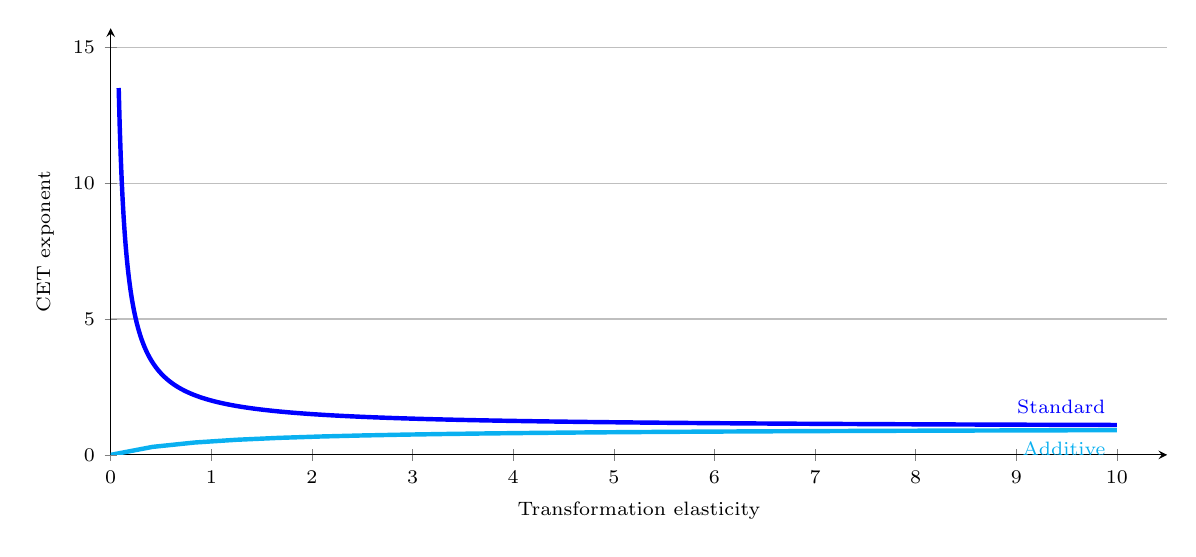
\begin{tikzpicture}[scale=1.0]
	\begin{axis}[axis lines=left,xtick={0,1.0,...,10.0},xmin=0,xmax=10.5,
ytick={0,5,...,15},ymin=0,ymax=15.7,
width=15cm,height=7cm,
x tick label style={
	/pgf/number format/.cd,
	fixed,
	fixed zerofill,
	precision=0,
	ymajorgrids,
	xlabel={\scriptsize{Transformation elasticity}},
	ylabel={\scriptsize{CET exponent}},
	/tikz/.cd
}]

\addplot[mark=none,blue,ultra thick,domain=0.08:10,samples=1000]{(x+1)/x} node[above left] {\scriptsize{Standard}} ;
\addplot[mark=none,ProcessBlue,ultra thick,domain=0:10]{x/(x+1)} node[below left] {\scriptsize{Additive}} ;

\end{axis}
\end{tikzpicture}
\end{figure}